%%%%%%%%%%%%%%%%%%%%%%%%%%%%%%%%%%%%%%%%%%%%%%%%%%%%%%%%%%%%%%%%%%%%%%
%%	Name: "Signal analysis template"
%%	File name: signalanalysis_template_main
%%	Version: 1.5
%%
%%	Compiler: XeLaTeX
%%
%%%%%%%%%%%%%%%%%%%%%%%%%%%%%%%%%%%%%%%%%%%%%%%%%%%%%%%%%%%%%%%%%%%%%%

\documentclass[conference,compsoc,onecolumn]{IEEEtran}

% *** LANGUAGE UTILITY PACKAGES ***
\usepackage[utf8]{inputenc} % Required for including letters with accents
\usepackage[spanish]{babel}

% *** USED PACKAGES ***
% *** MISC UTILITY PACKAGES ***
\usepackage{comment}			% Agregar comentarios
\usepackage{lipsum}				% Inserts dummy text
\usepackage{blindtext}
\usepackage{listings}					% Coding
\usepackage{verbatim}				% Verbatim
\usepackage[final]{pdfpages}
\usepackage{booktabs,dcolumn}
\usepackage{pdflscape}
\usepackage{afterpage}
%\setlist[itemize]{noitemsep, nolistsep}
\usepackage[bookmarks=false]{hyperref}
\usepackage{tcolorbox}									% Coloured boxes, for LATEX examples and theorems, etc
\usepackage{color}
\usepackage{xcolor} % Required for specifying colors by name									% Color packages foreground and back­ground color man­age­men
% *** CITATION PACKAGES ***
\usepackage{cite}
% *** GRAPHICS RELATED PACKAGES ***
\usepackage{graphicx}
\usepackage{caption}
\usepackage{pgfplots}
\usepackage{tikz}
\usetikzlibrary{shapes,arrows}
\usetikzlibrary{decorations.pathmorphing} % noisy shapes
\usetikzlibrary{fit}					% fitting shapes to coordinates
\usetikzlibrary{backgrounds}	% drawing the background after the foreground
\pgfplotsset{compat=1.13}
% *** MATH PACKAGES ***
\usepackage{amsmath}
\usepackage{mathtools}
\usepackage{amssymb}
\usepackage{amsfonts}
\usepackage{expl3}
\usepackage{bm}

% *** SPECIALIZED LIST PACKAGES ***
\usepackage{algorithmic}
\usepackage{listings}					% Coding
\usepackage[framed,numbered,autolinebreaks,useliterate]{mcode}
% *** ALIGNMENT PACKAGES ***
\usepackage{array}
% *** SUBFIGURE PACKAGES ***
%\ifCLASSOPTIONcompsoc
%\usepackage[caption=false,font=normalsize,labelfont=sf,textfont=sf]{subfig}
%\else
%\usepackage[caption=false,font=footnotesize]{subfig}
%\fi
% *** FLOAT PACKAGES ***
\usepackage{fixltx2e}
\usepackage{stfloats}
%\fnbelowfloat
%\usepackage{dblfloatfix}
% *** PDF, URL AND HYPERLINK PACKAGES ***
\usepackage{url}
\usepackage{everypage}


\usepackage{multirow} % In order to be able to insert rows spanning multiple lines
\usepackage{verbatim}
\usepackage[all]{xy}
\usepackage{listings}
\usepackage{subfigure}
\usepackage{multibib}
\usepackage{setspace} 
\usepackage{algorithm}			    	  % To insert nice algorithms

% *** CARPETA DONDE SE GUARDARAN LAS IMAGENES ***
\graphicspath{{figures/}}

% *** NUEVOS COMANDOS Y CONFIGURACIONES VARIAS ***
\interdisplaylinepenalty=2500
\newcommand{\Lpagenumber}{\ifdim\textwidth=\linewidth\else\bgroup
	\dimendef\margin=0
	\ifodd\value{page}\margin=\oddsidemargin
	\else\margin=\evensidemargin
	\fi
	\raisebox{\dimexpr -\topmargin-\headheight-\headsep-0.5\linewidth}[0pt][0pt]{%
		\rlap{\hspace{\dimexpr \margin+\textheight+\footskip}%
			\llap{\rotatebox{90}{\thepage}}}}%
	\egroup\fi}

\AddEverypageHook{\Lpagenumber}%

\newcommand{\newtxt}[1]{\textcolor{black}{#1}}
\renewcommand\IEEEkeywordsname{Palabras cláve:}
\newcommand{\mx}[1]{\mathbf{\bm{#1}}} % Matrix command
\newcommand{\vc}[1]{\mathbf{\bm{#1}}} % Vector command

%% Separación de palabras
\hyphenation{op-tical net-works semi-conduc-tor HHMMSS}


\begin{document}

% *** TITLES AND NAMES ***
% title of the document
\title{Plataforma de seguimiento de datos COVID-19 para Colombia.}
% author names and affiliations

\makeatletter
\newcommand{\linebreakand}{%
  \end{@IEEEauthorhalign}
  \hfill\mbox{}\par
  \mbox{}\hfill\begin{@IEEEauthorhalign}
}
\makeatother

\author{
    \IEEEauthorblockN{Janis~Andrea~Salazar~Sánchez}
    \IEEEauthorblockA{Escuela de Ciencias Exactas e Ingeniería\\
	    Universidad Sergio Arboleda - Bogotá, Colombia\\
	    janis.salazar01@correo.usa.edu.co}
    \and
    \IEEEauthorblockN{Valeria~Carvajal~Romero}
    \IEEEauthorblockA{Escuela de Ciencias Exactas e Ingeniería\\
	    Universidad Sergio Arboleda - Bogotá, Colombia\\
	    valeria.carvajal01@correo.usa.edu.co}
    \linebreakand
    \IEEEauthorblockN{Michael~Steven~Pinilla~Mateus}
    \IEEEauthorblockA{Escuela de Ciencias Exactas e Ingeniería\\
	    Universidad Sergio Arboleda - Bogotá, Colombia\\
	    michael.pinilla01@correo.usa.edu.co}
    
}

% *** MAKE TITLE ***
\maketitle
\IEEEoverridecommandlockouts
\IEEEpeerreviewmaketitle

\begin{abstract}
Como entrega de la primera y la segunda parte del proyecto de aula del curso Análisis de señales se desarrolla una plataforma que extrae los datos actualizados del COVID-19 presentados en
Colombia y la cuidad de Bogotá, tomando estos datos de la pagina web de datos del gobierno 'Datos Abiertos', y los guarda en una base de datos. Los datos posteriormente se representan
de forma selectiva mediante gráfica circular, gráficos de dos dimensiones y diagramas de barras. En este desarrollo se utiliza el lenguaje de programación python y el sistema de gestión de bases de datos SQLite.

\end{abstract}


\begin{IEEEkeywords}
COVID-19, Colombia, Bogotá, plataforma, seguimiento, pandemia
\end{IEEEkeywords}

\section{Antecedentes}
Dar cara a la pandemia ha sido un desafío para el sector de la salud y la epidemiología, para el personal que trabaja en primera línea y los que derivan en todo el mundo. La poca certidumbre, la atención dedicada a cada paciente y la precoz infraestructura y herramientas, los intentos de conseguir resultados e intervenciones optimos, la ansiedad, miedo y preocupacación colectiva, el desconocimiento sobre las consecuencias futuras en el organismo, además a la probabilidad que existe de muerte incrementa el pánico al contagio, que al dia de hoy, 2 de Noviembre del año 2020, se registra en Colombia el SARS-CoV-2  como la segunda causa de muerte. 
\medskip
Se tiene evidencia que el pulmón es uno de los órganos con mayor riesgo de sufrir complicaciones cronicas, donde hay perturbaciones en el proceso respiratorio, afectando la capacidad de realizar ejercicio, las necesidades de oxígeno y la calidad de vida. El "volver a la normalidad" que varios anhelan es una esperanza con muy bajas probabilidades de que ocurra. 
\label{sec:results}

\section{Bibliotecas utilizadas}
A continuación se describe brevemente las bibliotecas utilizadas en el desarrollo de la plataforma:

 \begin{table}[H]
    \centering
    \begin{tabular}[c]{| m{15em} | m{35em} |} 
     \hline
     \textbf{Biblioteca} & \textbf{Utilidad}\\
     \hline
      \textit{pandas} & Manipulación y análisis de datos para el lenguaje de programación Python. En particular, ofrece estructuras de datos y operaciones para manipular tablas y series temporales.\\ 
     \hline
      \textit{sqlite3} & Biblioteca con funciones que permiten gestionar una base de datos liviana que proporciona un sistema de administración para bases de datos relacionales y sin mucha configuración.\\
     \hline
      \textit{matplotlib.pyplot} & Es una colección de funciones de estilo comando que hacen que matplotlib funcione como MATLAB. Cada función pyplot realiza algún cambio en una figura: Por ejemplo, crea una figura, crea un area de trazado en una figura, traza algunas líneas en un area de trazado, decora el trazado con etiquetas, etc.  \\ 
     \hline
      \textit{os} & Proporciona funciones para interactuar con el sistema operativo. OS, viene bajo los módulos de utilidad estándar de Python. Este módulo proporciona una forma portátil de utilizar la funcionalidad dependiente del sistema operativo. \\
     \hline
    \end{tabular}
    \caption{Bibliotecas utilizadas de python en el desarrollo.}
    \label{table:ta}
    \end{table}

\label{sec:results}

\section{Resultados}
Como se puede observar en la siguiente gráfica se estima porcentualmente en que estado se encuentran las personas contagiadas por COVID-19 en Colombia, donde una gran parte de estas han logrado recuperarse con un porcentaje del 89.3\% del total de casos. A pesar de que los recuperados son una cifra significativa, esto no representa que sean inmunes o que no puedan volver a contagiarse, además de que aún no se tiene información de si puedan llegar a presentar secuelas u dolencias crónicas. El 5.6\% se encuentran en aislamiento obligatorio en sus casas mientras su organismo logra eliminar el virus. El 1.9\% están siendo atendidos por el personal de salud en centros hospitalarios donde un 0.2\% se encuentran gravemente, siendo atendidos en la unidad de cuidados intensivos (UCI). Aunque el porcentaje de fallecidos se pueda considerar bajo, del 3.1\%, hay que ser conscientes de que se habla de vidas, un total de 25,998 personas que han dejado de estar con nosotros.\\
Es de gran importancia mensionar que la gráfica encontrada a la derecha hace referencia de la correcciòn respectiva a cada una de las gráficas observadas, la correción se realizó con la actualización de los datos que pasaro de ser 800000 desde el 30 de Septiembre a 1000000 a hoy 2 de Noviembre del 2020.

\begin{figure}[htbp]
\centering
\subfigure[{Primera Imágen}.]{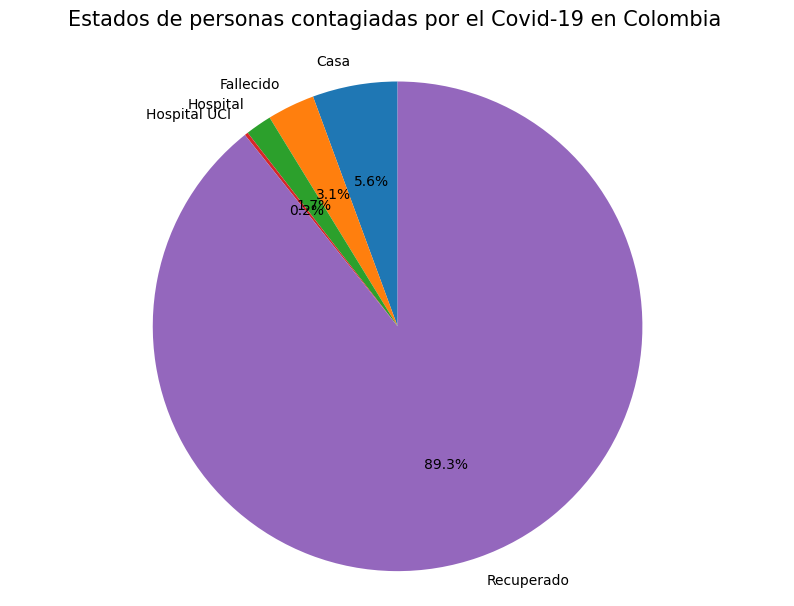
\includegraphics[width=60mm]{./images/GraficaCircular_Estados.png}}
\subfigure[{Corrección}.]{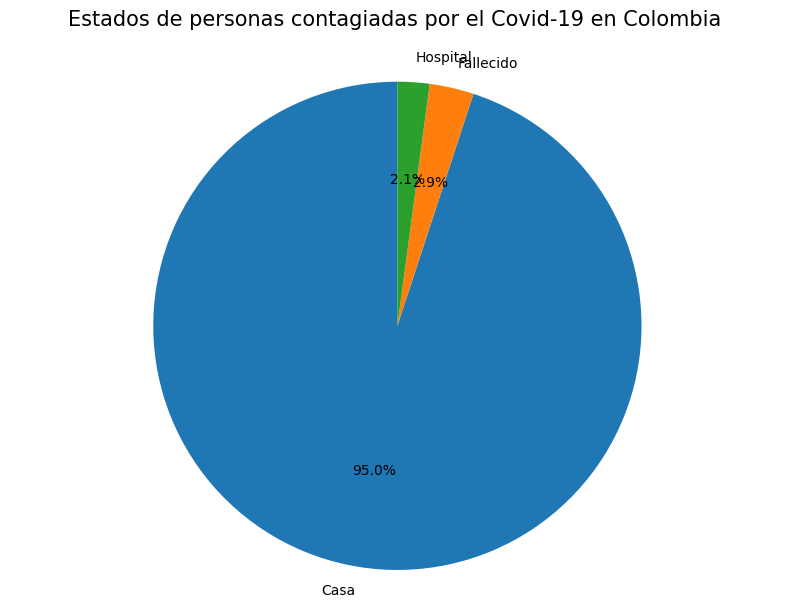
\includegraphics[width=60mm]{./12.png}}
\caption{Gráfica circular del estado de las personas con COVID-19 en Colombia.} \label{fig:lego}
\end{figure}

En la siguiente figura se puede evidenciar de manera clara la diferencia presentada entre la población de hombres y mujeres que se encuentran infectados actualmente de COVID-19 en Colombia, los valores se observan de manera porcentual y como resultado podemos concluir que la población masculina presenta mayores casos activos en un pequeño porcentaje de diferencia.\\

\begin{figure}[htbp]
\centering
\subfigure[{Primera Imágen}.]{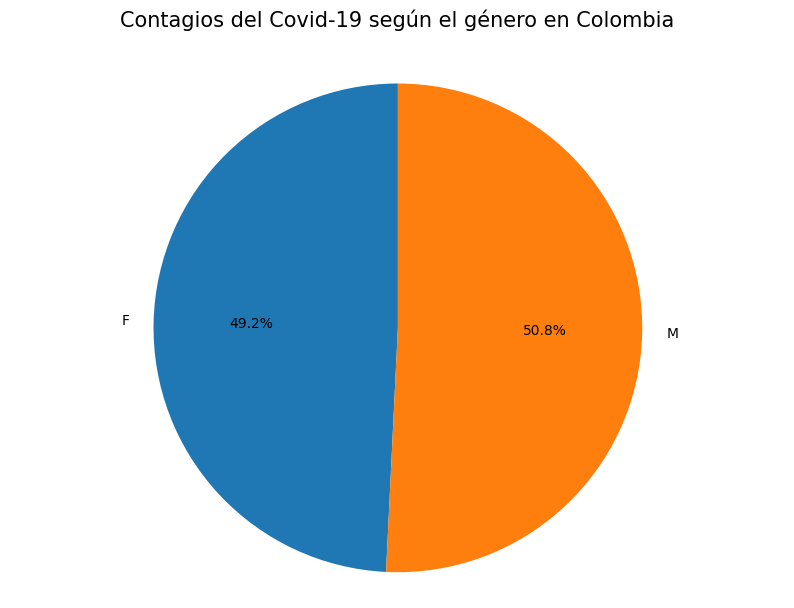
\includegraphics[width=60mm]{./images/GraficaCircular_Genero.png}}
\subfigure[{Corrección}.]{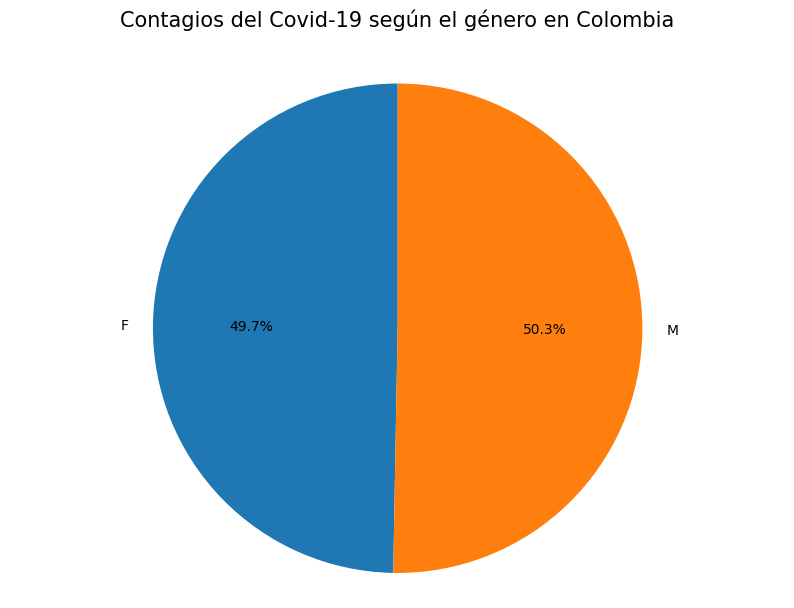
\includegraphics[width=60mm]{./GraficaCircular_Genero1.png}}
\caption{Gráfica circular de personas contagiadas con COVID-19 en Colombia según el sexo.} \label{fig:lego}
\end{figure}

Ahora, se representa a través de una gráfica de barras la cantidad de personas fallecidas clasificadas por su edad. Los contagiados que tuvieron una edad entre los 60 a 90 años de edad al momento de fallecimiento representan la mayoría, dando a entender que en este sector de la población existe una mayor tasa de letalidad en comparación con grupos de menor edad, representando una población más vulnerable. Aunque la mayor tasa de letalidad está en una edad avanzada, no quita la probabilidad de que niños, adolescentes, adultos jovenes y adultos estén en riesgo de morir por el virus del COVID-19.\\

\begin{figure}[htbp]
\centering
\subfigure[{Primera Imágen}.]{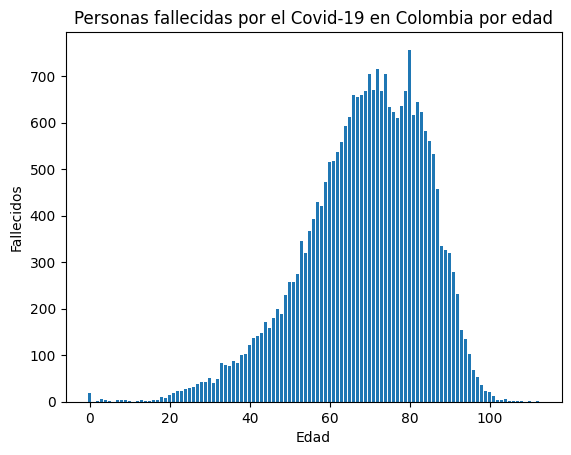
\includegraphics[width=60mm]{./images/GraficoBarras_Edad_Fallecidos.png}}
\subfigure[{Corrección}.]{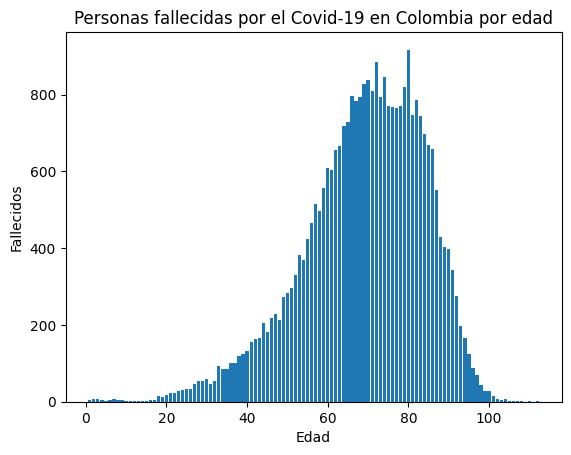
\includegraphics[width=60mm]{./GraficoBarras_Edad_Fallecidos1.png}}
\caption{Gráfica de barras de fallecimientos por COVID-19 en Colombia según la edad.} 
\label{fig:lego}
\end{figure}

A continuación, se tiene la gráfica de barras donde se realiza una comparación entre dos etnias, la indígena y la negra, obteniendo que mayormente hay contagiados en la etnia negra, casi a representar el doble de la indígena. Sin tener información relevante del porqué la etnia indígena conserva una cantidad minoritaria de contagiados, se puede aventurar a suponer que es debido a que su población es menor, ya que en Colombia ciertos grupos ilícitos y personal gubernamental toman como blanco de tiro a esta etnia.

\begin{figure}[H]
\centering
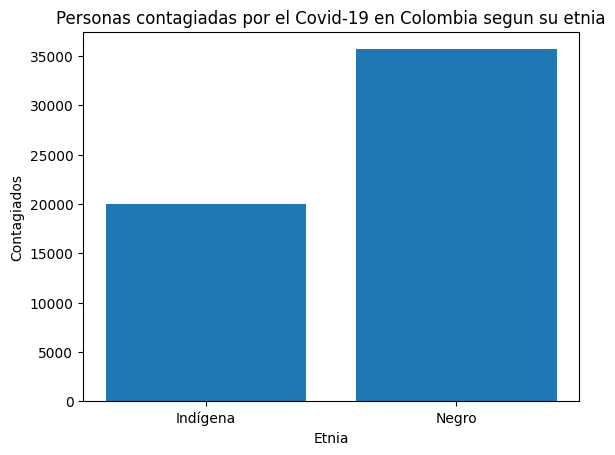
\includegraphics[width=8cm]{./images/GraficoBarras_Etnia_Contagios.png}
\caption{Gráfica de barras de contagiados por COVID-19 en Colombia según la etnia}
\label{fig:mesh1}
\end{figure}

En cuanto a los contagios por edad, se realiza una gráfica de dos dimensiones para visualizar la información, obteniendo que existe un mayor contagio en personas que rondan las edades entre los 30 a 50 años. Aunque este sector de la población representa la mayor tasa de contagio, no se llevan el título de mayor tasa de letalidad.


\begin{figure}[htbp]
\centering
\subfigure[{Primera Imágen}.]{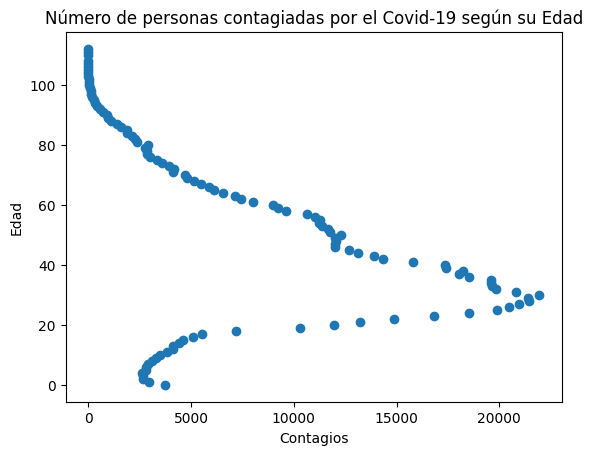
\includegraphics[width=60mm]{./images/Grafico2d_Edad.png}}
\subfigure[{Corrección}.]{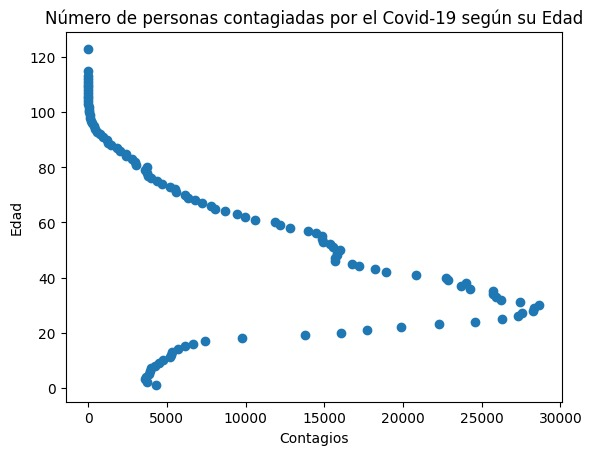
\includegraphics[width=60mm]{./images/2vichada.jpeg}}
\caption{Gráfica 2D de contagiados por COVID-19 en Colombia según la edad} 
\label{fig:lego}
\end{figure}

Para finalizar, se hace un análisis más localizado en el departamento de Vichada, obteniendo que en sus principales 4 ciudades (Santa Rosalía, Puerto Carreño, La Primavera y Cumaribo) existe un muy bajo número de contagiados reportados, excepto en su capital, Puerto Carreño, que si resalta entre sus vecinas con un número de aproximadamente 400 contagios.  

\begin{figure}[htbp]
\centering
\subfigure[{Primera Imágen}.]{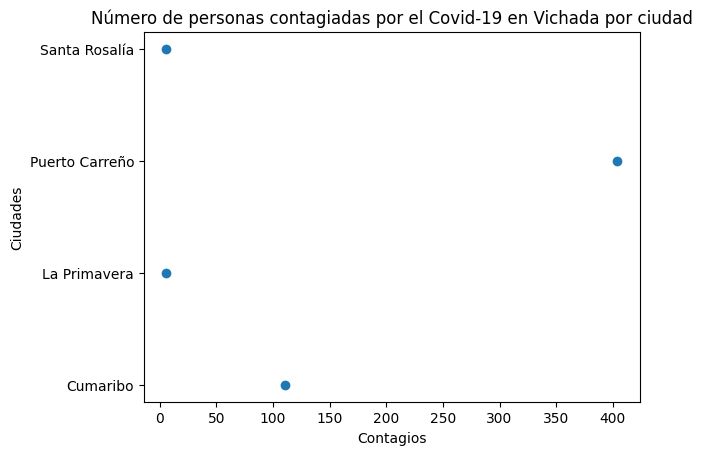
\includegraphics[width=60mm]{./images/Grafico2d_Vichada.png}}
\subfigure[{Corrección}.]{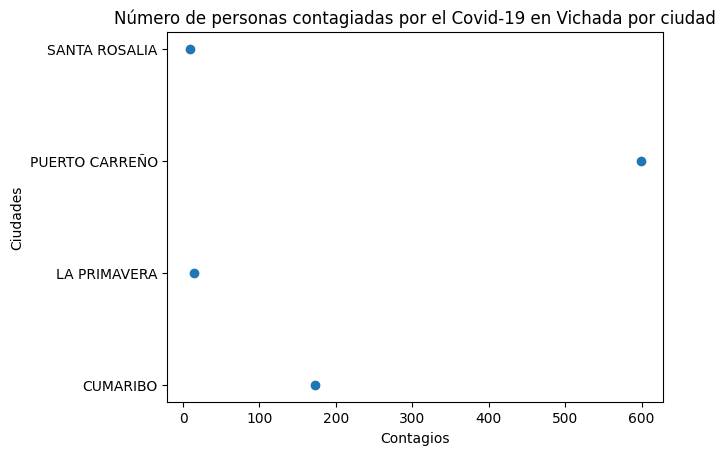
\includegraphics[width=60mm]{./Grafico2d_Vichada1.png}}
\caption{Gráfica 2D de contagiados por COVID-19 en Colombia localizados en las ciudades del departamento de Vichada.} 
\label{fig:lego}
\end{figure}

\section{Conclusiones de la primera entrega}
A continuación se resume las conclusiones basadas en los resultados obtenidos: 
\label{sec:conclusions}
\begin{itemize}
    
    \item La población masculina presenta mayores casos activos en un pequeño porcentaje de diferencia respecto a las mujeres.
    \item Los contagiados que tienen una edad entre los 60 a 90 años de edad tienen la mayor tasa de letalidad en comparación con grupos de menor edad. 
    \item Una gran parte de personas han logrado recuperarse del COVID-19 con un porcentaje del 89.3\% del total de casos. El 5.6\% se encuentran en aislamiento obligatorio. El 1.9\% están siendo atendidos por el personal de salud en centros hospitalarios donde un 0.2\% se encuentran en UCI y el porcentaje de fallecidos es del 3.1\%.
    \item Entre las etnias indígena y negra, existe mayor número de contagios en la etnia negra, casi representando el doble de la indígena.
    \item Las personas que rondan las edades entre los 30 a 50 años representa la mayor tasa de contagio.
    \item En el departamento de Vichada existe un muy bajo número de contagiados reportados, excepto en su capital, Puerto Carreño.
    
\end{itemize}

\section{Segunda parte del proyecto}

Ahora, los datos del COVID-19 presentes en Colombia y Bogotá se representan en un mapa de acuerdo a las localidades. Estos datos, se discriminan por: evolución de casos positivos, sexo, edad y localidad. Para esto, se descarga nueva información y se almacena en una nueva base de datos para los datos de Bogotá específicamente, y se agrega gráfica de tiempo.

\medskip

Para empezar, se toma los datos del COVID-19 de la capital de Colombia, Bogotá D.C, se procesan los datos obteniendo las siguientes gráficas:

\smallskip

A continuación, se observa como varía la cantidad de contagiados a través del tiempo, llegando al pico en el instante de tiempo 8-13 teniendo una cantidad considerable de contagiados por encima  de las 700 personas: 
\begin{figure}[H]
\centering  
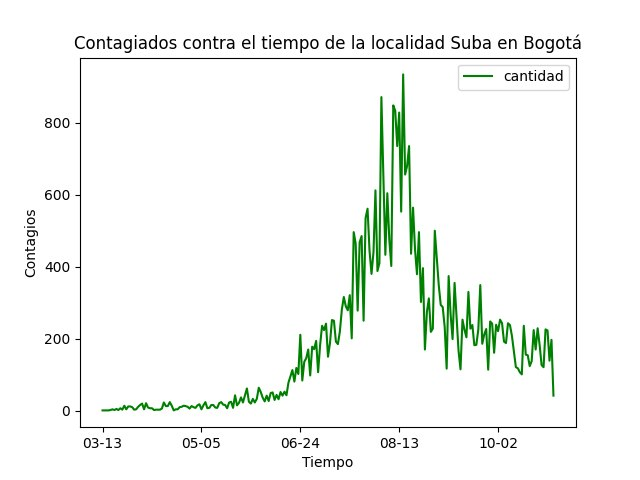
\includegraphics[width=8cm]{./images/contagiosSuba.jpg}
\caption{Contagiados vs tiempo localidad de Suba, Bogotá D.C}
\label{fig:mesh1}
\end{figure}

\smallskip

En esta gráfica, se segmenta las localidades de Bogotá para visualizar dónde se encuentra la mayor fuente de contagios para los hombres, dando como resultado la localidad de Suba y Kennedy que superan los 20000 de contagios. Al contrario, la localidad de la Candelaria y los Mártires se conservan como dos de las localidades donde el contagio ha sido considerablemente menor, por debajo de los 4000.  

\begin{figure}[H]
\centering  
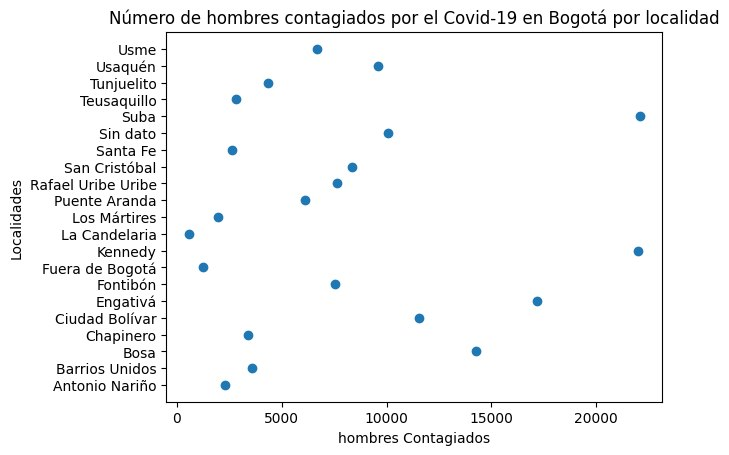
\includegraphics[width=8cm]{./images/hombresLocalidad.jpg}
\caption{Número de hombres contagiados en Bogotá por localidad}
\label{fig:mesh1}
\end{figure}

\smallskip

Como se mencionó anteriormente, la localidad de Kennedy es una localidad donde se encuentra en el top de contagios a hombres. Ahora, queriendo comparar esto con las mujeres se obtiene que la población femenina es aún mayor, dando a entender que la localidad de Kennedy es en general una localidad donde se encuentran muchos contagiados por el COVID-19. 

\begin{figure}[H]
\centering  
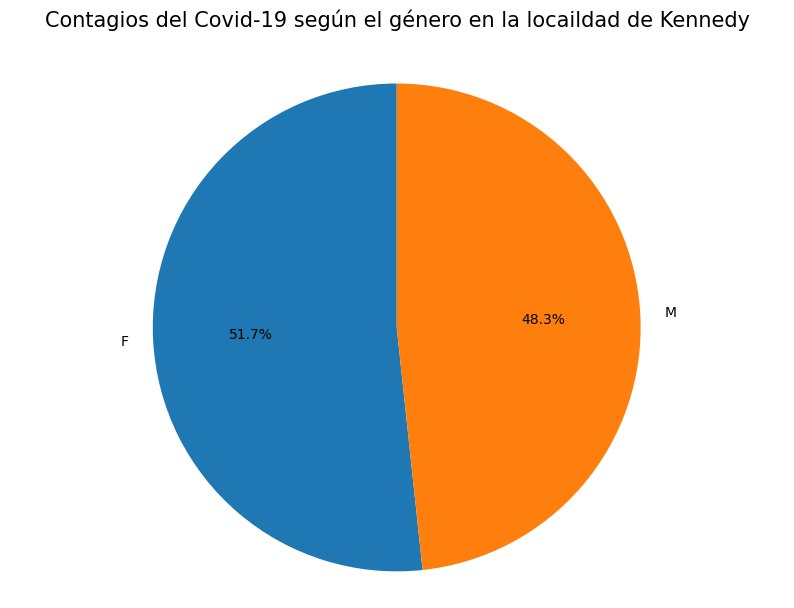
\includegraphics[width=8cm]{./images/kennedy.jpg}
\caption{Contagios según el genero en la localidad de Kennedy}
\label{fig:mesh1}
\end{figure}

\smallskip

En la siguiente, se muestra los fallecidos por localidad, dando confirmación a la premisa dicha anteriormente que Kennedy es la localidad com mayor contagios, superando los 1000, luego sigue Engativa y Suba superando los 800 contagios. En el otro extremo, se encuentra La Candelaria y los Mártires por debajo de los 200 contagios.
\begin{figure}[H]
\centering  
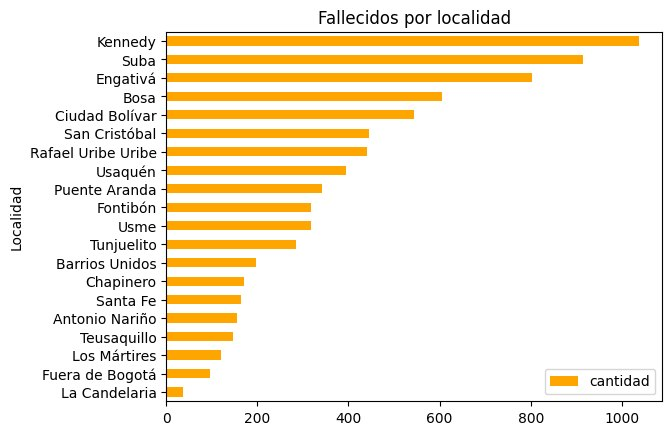
\includegraphics[width=8cm]{./images/fallecidosLocalidad.jpg}
\caption{Fallecidos por localidad - Bogotá D.C}
\label{fig:mesh1}
\end{figure}



En la gráfica siguiente se observa las personas que han sido recuperadas en Colombia por Covid-19 de dos formas distintas las cuales son: PCR, la cual es una prueba de diagnostico que permite confirmar la infección y la otra manera observada en la gráfica es la recuperación gradual del individuo con el paso del tiempo, la cual es la manera con mayor porcentaje.
\begin{figure}[H]
\centering
\includegraphics[width=8cm]{./GraficoBarras_Recuperacion1.png}
\caption{Gráfica de Barras de personas recuperadas en Colombia}
\label{fig:mesh1}
\end{figure}

Como se puede observar en la gráfica presentada a continuación se tiene el porcentaje de cada uno de los contagios presentes a través del paso del tiempo, se puede concluir que este tiene un valor sercano a los 11.000 contagios.
\begin{figure}[H]
\centering
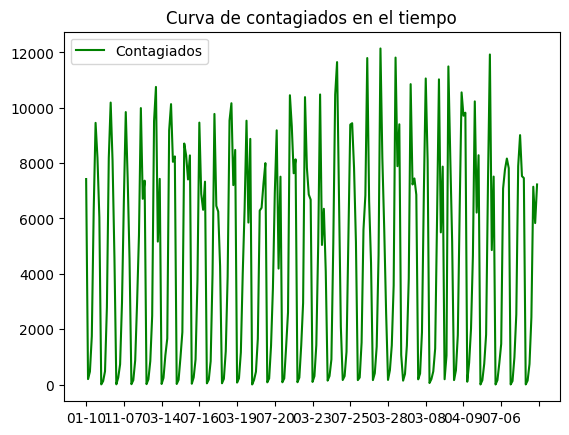
\includegraphics[width=8cm]{./Graficocontagios1.png}
\caption{Gráfica de Contagios vs tiempo.}
\label{fig:mesh1}
\end{figure}

Esta gráfica nos da un buen alivio con respecto a la mortalidad que se presenta en el pais, puesto que el valor de las personas recuperadas es mayor en grandes proporciones, lo cual nos permite concluir que el valor de personas que lastimosamente fallecen por el contagio del Covid-19 es relativamente pequeño con referente a los esfuerzo que se realiza por parte de las entidades medicas y los mismos ciudadanos para que esta situación no sea de esta manera.
\begin{figure}[H]
\centering
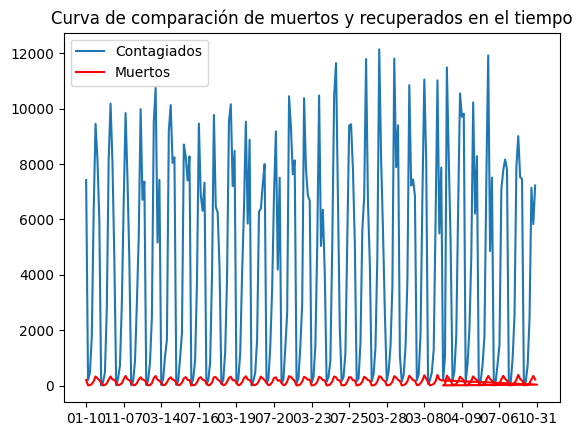
\includegraphics[width=8cm]{./Graficomuerte2.png}
\caption{Gráfica de Numero de personas recuperados vs fallecidos.}
\label{fig:mesh1}
\end{figure}

En el departamento de Risaralda se realizó un estudio de cuantas personas fallecian por cuidad, en donde encontramos que la cuidad que presenta mayores indices de mortalidad es Pereira con mas de 250 personas, teniendo una gran diferencia con las demas ciudades las cuales presentan maximo 50 fallecidos.
\begin{figure}[H]
\centering
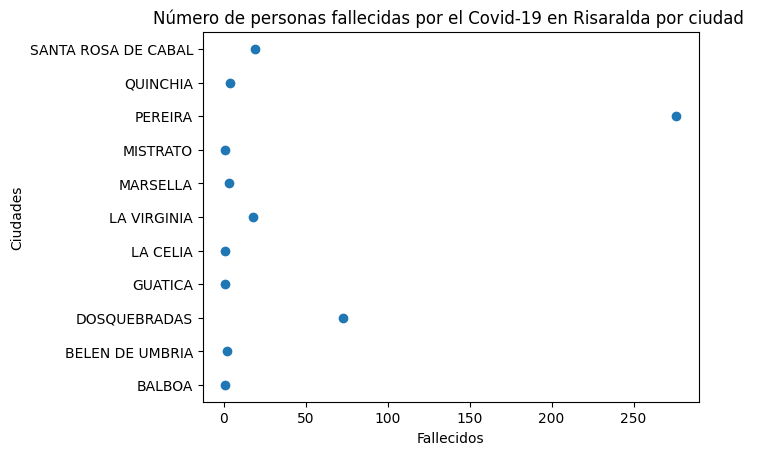
\includegraphics[width=10cm]{./Grafico_Depto1.png}
\caption{Gráfica de Numero de personas fallecidas en Risaralda.}
\label{fig:mesh1}
\end{figure}

Estos datos se deberán representar en un .
\section{Mapa de Colombia y de Bogotá de acuerdo a los departamentos y localidades}

Ahora, se representan los datos del COVID-19 en un mapa de calor de Colombia y Bogotá, teniendo como resultado las siguientes figuras:

\medskip

Como se observa según el degrade de color presente en la figura Bogotá es uno de los lugares mayormente \verb|"|contaminados\verb|"| por el virus.
\begin{figure}[H]
\centering
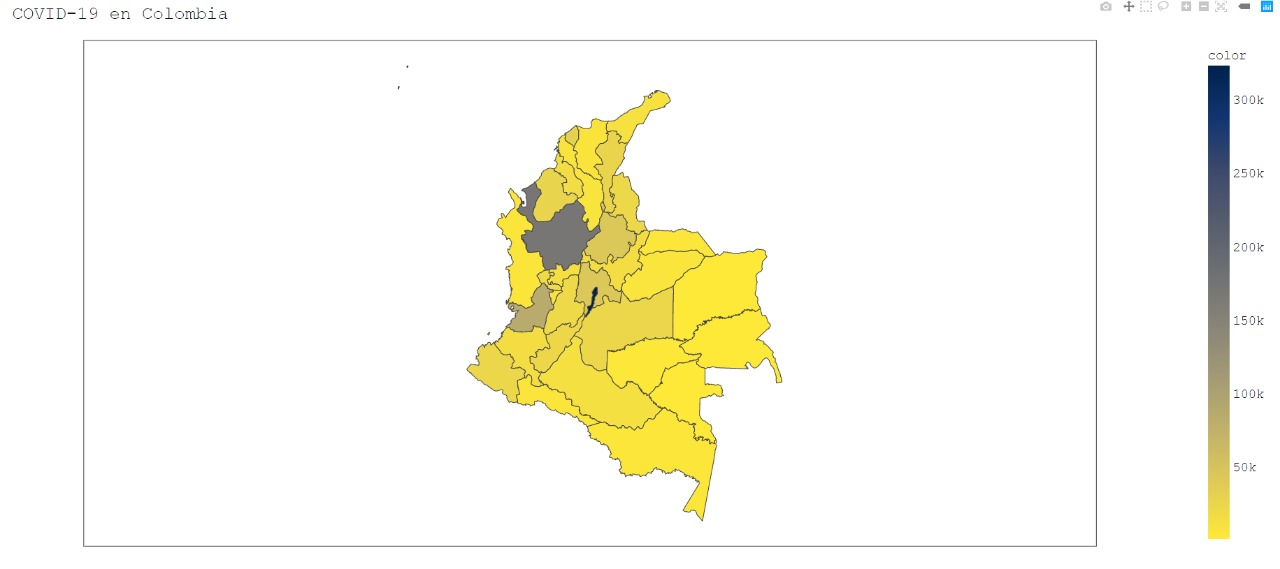
\includegraphics[width=18cm]{./images/colombia.jpeg}
\caption{Mapa de calor de Colombia.}
\label{fig:mesh1}
\end{figure}
Esta figura la puede descargar en formato html llendo al repositorio Git que se encuentra al final del informe.

\medskip

La siguiente figura es el mapa de calor de Bogotá segmentado en localidades, donde se evidencia que Suba y Kennedy son un gran foco del virus, estos representados en color amarillo.

\begin{figure}[H]
\centering
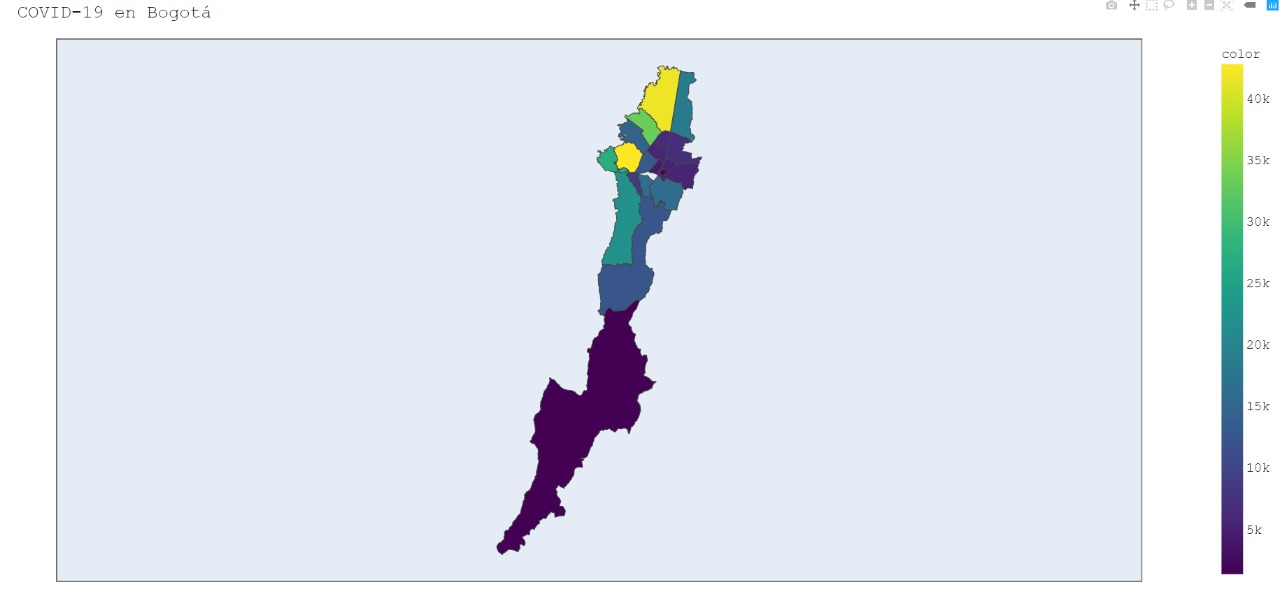
\includegraphics[width=18cm]{./images/bogota.jpeg}
\caption{Mapa de calor de Bogotá.}
\label{fig:mesh1}
\end{figure}
Esta figura la puede descargar en formato html yendo al repositorio Git que se encuentra al final del informe.

\medskip

A continuación se expondran las bibliotecas trabajadas para poder realizar la elaboracion de las gráficas de calor.

\begin{table}[H]
    \centering
    \begin{tabular}[c]{| m{15em} | m{35em} |} 
     \hline
     \textbf{Biblioteca} & \textbf{Utilidad}\\
     \hline
      \textit{pandas} & Manipulación y análisis de datos para el lenguaje de programación Python. En particular, ofrece estructuras de datos y operaciones para manipular tablas y series temporales.\\ 
     \hline
      \textit{matplotlib.pyplot} & Es una colección de funciones de estilo comando que hacen que matplotlib funcione como MATLAB. Cada función pyplot realiza algún cambio en una figura: Por ejemplo, crea una figura, crea un area de trazado en una figura, traza algunas líneas en un area de trazado, decora el trazado con etiquetas, etc.  \\ 
     \hline
      \textit{os} & Proporciona funciones para interactuar con el sistema operativo. OS, viene bajo los módulos de utilidad estándar de Python. Este módulo proporciona una forma portátil de utilizar la funcionalidad dependiente del sistema operativo. \\
     \hline
      \textit{Request} & API es un API simple significa que todas las formas the peticiones HTTP son obvias y trae el URL de la base de datos y lo guarda como un formato CSV.\\
      \hline
      \textit{Plotly.Express} & Contiene funciones que pueden crear figuras completas a la vez, y se denomina Plotly Express o PX. Plotly Express es una parte integrada de la plotlybiblioteca y es el punto de partida recomendado para crear las figuras más comunes.\\
      \hline
      \textit{Plotly} & Es una plataforma moderna para el trazado y visualización de datos. Útil para producir una variedad de gráficos, especialmente para ciencias de datos.\\
      \hline
      \textit{Geopandas} & Es la implementación geoespacial de la librería de Python llamada Pandas, esta librería está enfocado en el cálculo masivo bajo el enfoque de "Big Data". GeoPandas permite el uso de los tipos de datos de Pandas para las operaciones espaciales de tipos geométricos de SIG (puntos, líneas y polígonos).\\
      \hline
      \textit{Numpy} & Es una biblioteca para el lenguaje de programación Python que da soporte para crear vectores y matrices grandes multidimensionales, junto con una gran colección de funciones matemáticas de alto nivel para operar con ellas.\\
      \hline
    \end{tabular}
    \caption{Bibliotecas utilizadas de python en el desarrollo.}
    \label{table:ta}
    \end{table}
    
\section{Conclusiones de la segunda entrega}
A continuación se resume las conclusiones basadas en los resultados obtenidos: 
\label{sec:conclusions}
\begin{itemize}
    
    \item El 29,9 \verb|%|de los casos reportados en Colombia de Covid-19, se encuentran en Bogotá D.C. (corte 31-10-2020). En la ciudad, se han presentado 321.596 casos confirmados de los cuales 2.191 son casos nuevos; del total de casos 51,6\verb|%| son mujeres y la mayor concentración de casos de acuerdo con la edad, está entre los 20 a 49 años con un peso porcentual de 60,9\verb|%|.
    
    \item La localidad de Kennedy registra el 14,1\verb|%| de los casos de la ciudad ( 42.551), Suba el 13,8\verb|%| (41.533), Engativá el 11,0\verb|%| (33.111), Bosa el 8,9\verb|%| (26.952) y Ciudad Bolívar el 7,3\verb|%| (21.882); estas cinco localidades aportan el 55,1\verb|%| de los casos confirmados en el Distrito, cabe aclarar que se evidencian 20.411 registros “Sin dato” en la variable localidad, porque aún se encuentran en investigación epidemiológica. El 5,4\verb|%| de los casos se encuentran en un estado leve, el 1,1\verb|%| moderado, el 0,2\verb|%| en estado grave. Del total de los casos, 38,9\verb|%| (125.030) no presentaron síntomas. Se han recuperado 291.598 personas (90,7\verb|%|) y han fallecido 7.650 (2,4\verb|%|). El 98,2\verb|%| de los casos se encuentran en casa, el 1,7\verb|%| en hospitalización general y el 0,2\verb|%| en Unidades de Cuidado Intensivo-UCI.
    
    \item Bogotá tiene 266,7 casos activos de Covid-19 por cada 100.000 habitantes, así como una tasa de mortalidad por COVID – 19 en hombres de 123,2 por cada 100.000 habitantes y en mujeres 61,3 por cada 100.000 habitantes. Del total de unidades de cuidado intensivo destinadas para Covid-19, el 51,1\verb|%| están ocupadas. Al comparar Bogotá con las principales ciudades de América latina, Miami, Nueva York y Madrid, ocupamos el lugar 6 con 41.246 casos por 1 millón de habitantes.
    
\end{itemize}

\section{Repositorio GIT}
En el siguiente link se encuentra el repositorio GIT que se utilizó para el desarrollo de la plataforma:
\begin{itemize}
\item https://github.com/Vaal-01/COVID-Colombia
\end{itemize}

\nocite{*}
\bibliographystyle{IEEEtran}
\label{sec:biblio}
% Descomente y modiffique el archivo biblio.bib para agregar bibliografía
\bibliography{bib/biblio} 





%\pagestyle{empty}
\end{document}

